% Options for packages loaded elsewhere
\PassOptionsToPackage{unicode}{hyperref}
\PassOptionsToPackage{hyphens}{url}
%
\documentclass[
  12pt,
]{article}
\usepackage{amsmath,amssymb}
\usepackage{lmodern}
\usepackage{iftex}
\ifPDFTeX
  \usepackage[T1]{fontenc}
  \usepackage[utf8]{inputenc}
  \usepackage{textcomp} % provide euro and other symbols
\else % if luatex or xetex
  \usepackage{unicode-math}
  \defaultfontfeatures{Scale=MatchLowercase}
  \defaultfontfeatures[\rmfamily]{Ligatures=TeX,Scale=1}
\fi
% Use upquote if available, for straight quotes in verbatim environments
\IfFileExists{upquote.sty}{\usepackage{upquote}}{}
\IfFileExists{microtype.sty}{% use microtype if available
  \usepackage[]{microtype}
  \UseMicrotypeSet[protrusion]{basicmath} % disable protrusion for tt fonts
}{}
\makeatletter
\@ifundefined{KOMAClassName}{% if non-KOMA class
  \IfFileExists{parskip.sty}{%
    \usepackage{parskip}
  }{% else
    \setlength{\parindent}{0pt}
    \setlength{\parskip}{6pt plus 2pt minus 1pt}}
}{% if KOMA class
  \KOMAoptions{parskip=half}}
\makeatother
\usepackage{xcolor}
\usepackage[margin=1in]{geometry}
\usepackage{graphicx}
\makeatletter
\def\maxwidth{\ifdim\Gin@nat@width>\linewidth\linewidth\else\Gin@nat@width\fi}
\def\maxheight{\ifdim\Gin@nat@height>\textheight\textheight\else\Gin@nat@height\fi}
\makeatother
% Scale images if necessary, so that they will not overflow the page
% margins by default, and it is still possible to overwrite the defaults
% using explicit options in \includegraphics[width, height, ...]{}
\setkeys{Gin}{width=\maxwidth,height=\maxheight,keepaspectratio}
% Set default figure placement to htbp
\makeatletter
\def\fps@figure{htbp}
\makeatother
\setlength{\emergencystretch}{3em} % prevent overfull lines
\providecommand{\tightlist}{%
  \setlength{\itemsep}{0pt}\setlength{\parskip}{0pt}}
\setcounter{secnumdepth}{-\maxdimen} % remove section numbering
\usepackage{booktabs}
\usepackage{longtable}
\usepackage{array}
\usepackage{multirow}
\usepackage{wrapfig}
\usepackage{float}
\usepackage{colortbl}
\usepackage{pdflscape}
\usepackage{tabu}
\usepackage{threeparttable}
\usepackage{threeparttablex}
\usepackage[normalem]{ulem}
\usepackage{makecell}
\usepackage{xcolor}
\ifLuaTeX
  \usepackage{selnolig}  % disable illegal ligatures
\fi
\IfFileExists{bookmark.sty}{\usepackage{bookmark}}{\usepackage{hyperref}}
\IfFileExists{xurl.sty}{\usepackage{xurl}}{} % add URL line breaks if available
\urlstyle{same} % disable monospaced font for URLs
\hypersetup{
  pdftitle={Prediction of Breast Cancer Survival using Machine Learning Techniques},
  pdfauthor={Ye Yao, Zhilin Zhang, Hengde Ouyang},
  hidelinks,
  pdfcreator={LaTeX via pandoc}}

\title{Prediction of Breast Cancer Survival using Machine Learning
Techniques}
\author{Ye Yao, Zhilin Zhang, Hengde Ouyang}
\date{12/17/2022}

\begin{document}
\maketitle

\hypertarget{introduction}{%
\section{Introduction}\label{introduction}}

Breast cancer is the most common cancer among women in the United
States. According to the survey, the average risk of a woman in the
United States developing breast cancer is about 13\%{[}1{]}. The
survival prediction, especially 5-year survival analysis, was largely
used to help doctors understand the prognosis, predict treatment
efficiency and develop individualized treatment plans. In previous
studies, machine learning was largely applied for its high accuracy and
fewer assumption requirements. In this study, the survival prediction
model was built based on data with 300998 cases and 9 variables
extracted from the SEER research database.

\hypertarget{data-description}{%
\section{Data Description}\label{data-description}}

Nine variables with potential effects on survival were selected,
including Age, Race, ER\_PR, HER, Tumor Size, surgery, sex, Reginal and
Stage. The Race was categorized into Asian, Black, White, America
Indian, Native Hawaii and other Pacific islanders and others. ER\_PR,
the score of estrogen receptor/progesterone receptor tests. was
reflected as 0, 1, 2, indicating ER-/PR-, ER+/PR- or ER-/PR+, ER+/PR+.
And receiving surgery of removing the tissue in the primary site was
also represented as Surgery.And variable Reginal reflects the existence
of positive lymph nodes. In addition, there was an interaction term
between Tumor Size and Reginal. The outcome variable is survival time in
months.

\hypertarget{data-preprocessing}{%
\section{Data Preprocessing}\label{data-preprocessing}}

Data from 2004-2014 was treated as train data while data from 2015 was
treated as test data. Multivariate imputation by chained equations
(MICE) was used to impute the covariates, assuming that the missing data
were missing at random (MAR). Incomplete variables were imputed by
separate models, including predictive mean matching for numeric
variables, logistic regression for binary variables, bayesian polytomous
regression for factor variables, and proportional odds model for ordinal
variables. There are 93617 cases in the complete data after mice
imputation.

\hypertarget{method}{%
\section{Method}\label{method}}

Survival analysis is known to explore the occurrence of an event of
interest, such as alive, death or recurrence. In this study, the years
of survival were calculated from the date of diagnosis to the date of
death. Patients' five years of survival status is the main interest,
only patients dead 5 years after diagnosis or lost follow-up would be
considered. Among the total of 94326 patients, 74313 were alive after
five years of diagnosis, 658 were censored and 20013 were dead. The
survival package was used to plot the stratified survival curve for each
important categorical variable of interest to identify its impacts on
the survival rate. Based on the Kaplan-Meier plots and the descriptive
analysis, two predicting models were constructed.

Cox regression analysis was used to estimate hazard ratios (HRs), 95\%
confidence intervals and p-values. The study used a Forest plot to
specify the efficiency of predicting variables. To observe the patient's
5-year survival rate, we used the ``rms'' package to build a model for
the filtered variables and draw a nomogram to visualize the prediction
results of the independent variables and survival outcomes.

The random survival forest takes the binary survival tree as the basic
unit and is an extension of the traditional binary decision tree. When
the input data passes through the nodes of the binary decision tree, it
will be divided into two groups of data by the judgment conditions of
the nodes until the input data are classified into the same category.
Unlike the usual decision tree, the survival decision tree uses a
log-rank test to determine the splits. The study first constructed a
random survival forest with 100 decision trees. Based on the decreasing
rate of error, 50 trees were determined to build our model. The
information on the RSF model is given in the table.

The efficiency of the prediction model was measured by the concordance
index(C-index) and out-of-bag error rate (OOB error rate). The
discrimination between the prediction value and the real value was
calculated by C-index using the ``pec'' package. OOB error is a method
of measuring the prediction error utilizing bootstrap aggregating
(bagging). Bagging uses sub-sampling with replacement to create training
samples for the model to learn from. OOB error is the mean prediction
error on each training sample xi, using only the trees that did not have
xi in their bootstrap sample. The OOB error rate of RSF is given
straight from the model function and the study imitated the bootstrap 50
times to get the average OOB error rate for Cox regression. The model
with a high C-index value and a low OOB error rate was considered to be
efficient.

\hypertarget{result}{%
\section{Result}\label{result}}

\hypertarget{cox-proportional-hazard-model}{%
\subsubsection{Cox Proportional Hazard
Model}\label{cox-proportional-hazard-model}}

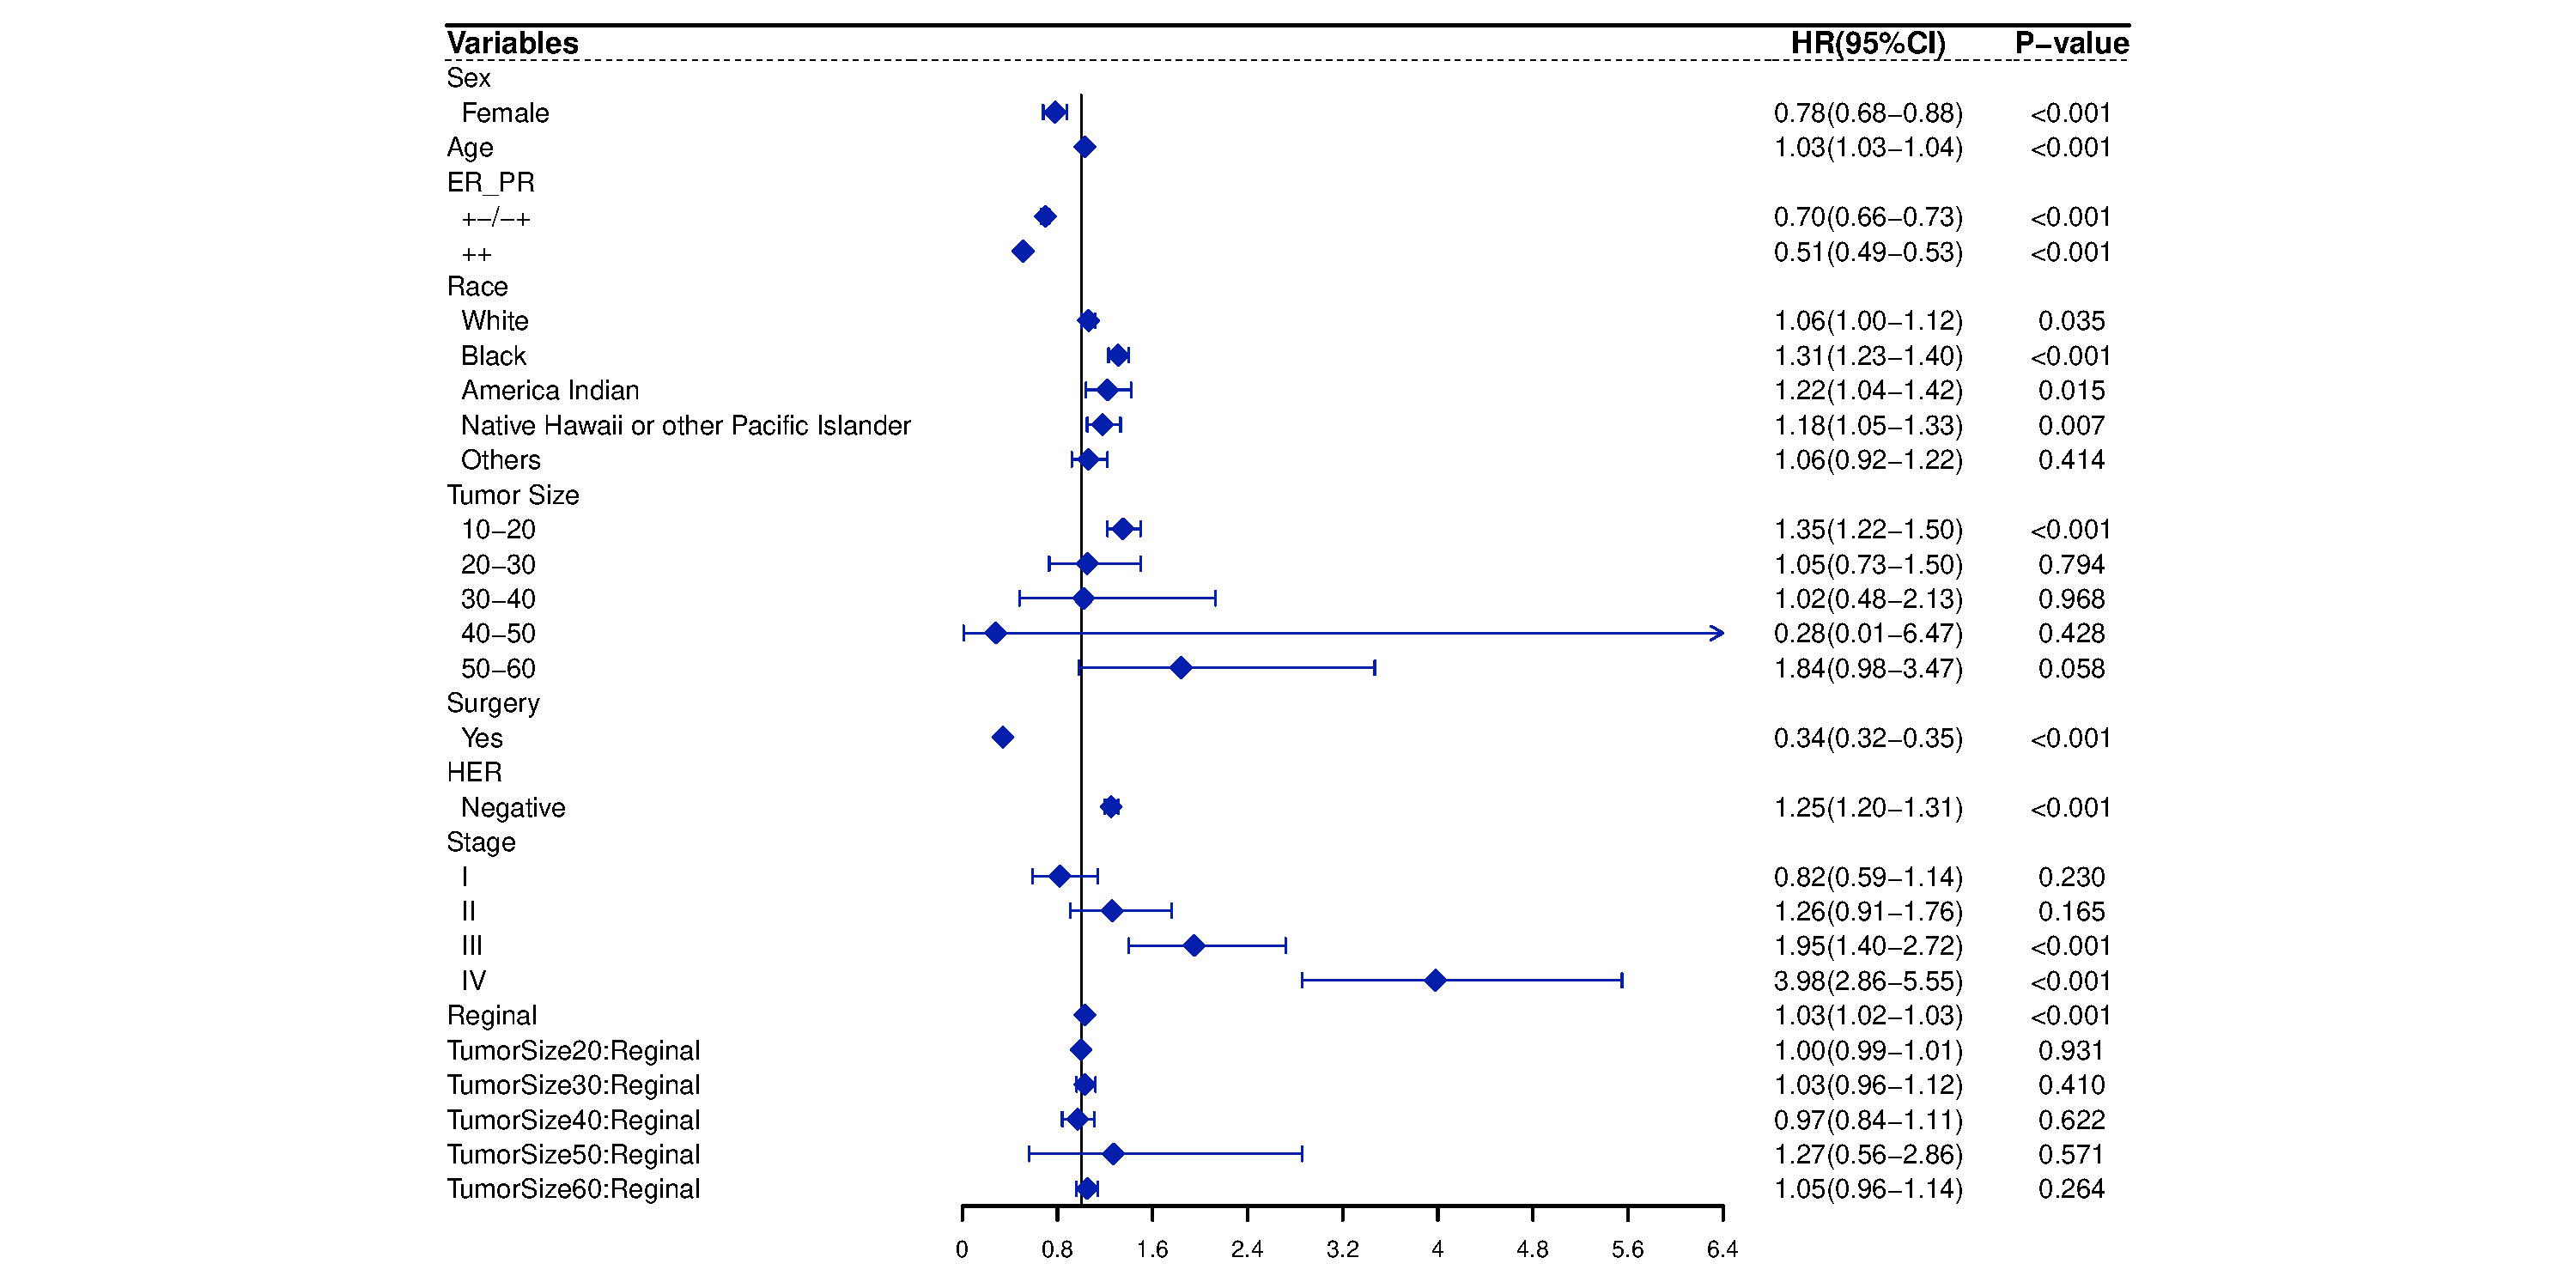
\includegraphics{report_files/figure-latex/unnamed-chunk-2-1.pdf}

Adjusting for other variables, it was determined that the key predictor
variables influencing survival probability includes sex (HR=0.78,
95\%CI={[}0.68,0.88{]}), age(HR=1.03, 95\% CI={[}1.03,1.04{]}), all
groups in ER\_PR(HR=0.70, 95\% CI={[}0.66,0.73{]} and HR=0.51,95\%
CI={[}0.49,0.53{]}), surgery (HR=0.34, 95\% CI={[}0.32,0.35{]}), and
HER2 (HR=1.25, 95\%CI={[}1.20,1.31{]}).

For binary variables, females were predicted to have longer survival
time than males. Receiving surgery or a positive HER2 test result also
indicate a higher chance of survival. For the continuous variables, it
was observed the predicted survival time decreases as age increases. And
patients with more ER and PR tests being positive were predicted to have
a longer survival time.

What's more, for categorical variables, the relationship between
survival months and each variable becomes more complicated. Compared to
the reference group, stage I (HR=0.82, 95\% CI={[}0.59,1.14{]}) and
stage II (HR=1.26, 95\% CI={[}0.97,1.76{]}) were observed to be
insignificant. However, patients at stage III(HR=1.95, 95\%
CI={[}1.40,2.72{]}) and IV (HR=3.98, 95\% CI={[}2.86,5.55{]}) were
predicted to have shorter survival time. Especially in stage IV, the
hazard ratio increases dramatically.

The effect of tumor size on survival months is also complicated.
Compared to the reference group, a tumor size of 40-50mm (HR=0.28,
95\%CI={[}0.01,6.47{]}) and a tumor size of 50-60mm (HR=1.84, 95\%
CI={[}0.98,3.47{]}) has an positive effect on survival months, which is
inconsistent with previous study. And the interaction term between Tumor
Size and Reginal was still insignificant.

Lastly, by comparing survival months among different races, Asian is
treated as the reference group. Black (HR=1.31, 95\%
CI={[}1.23,1.40{]}), White (HR=1.06, 95\% CI={[}1.00,1.12{]}), America
Indian(HR=1.22, 955CI={[}1.04, 1.42{]} and Native Hawaii and other
Pacific islanders (HR=1.18, 95\% CI={[}1.05,1.33{]}) have a
significantly higher hazard ratio, reflecting a higher risk of death.

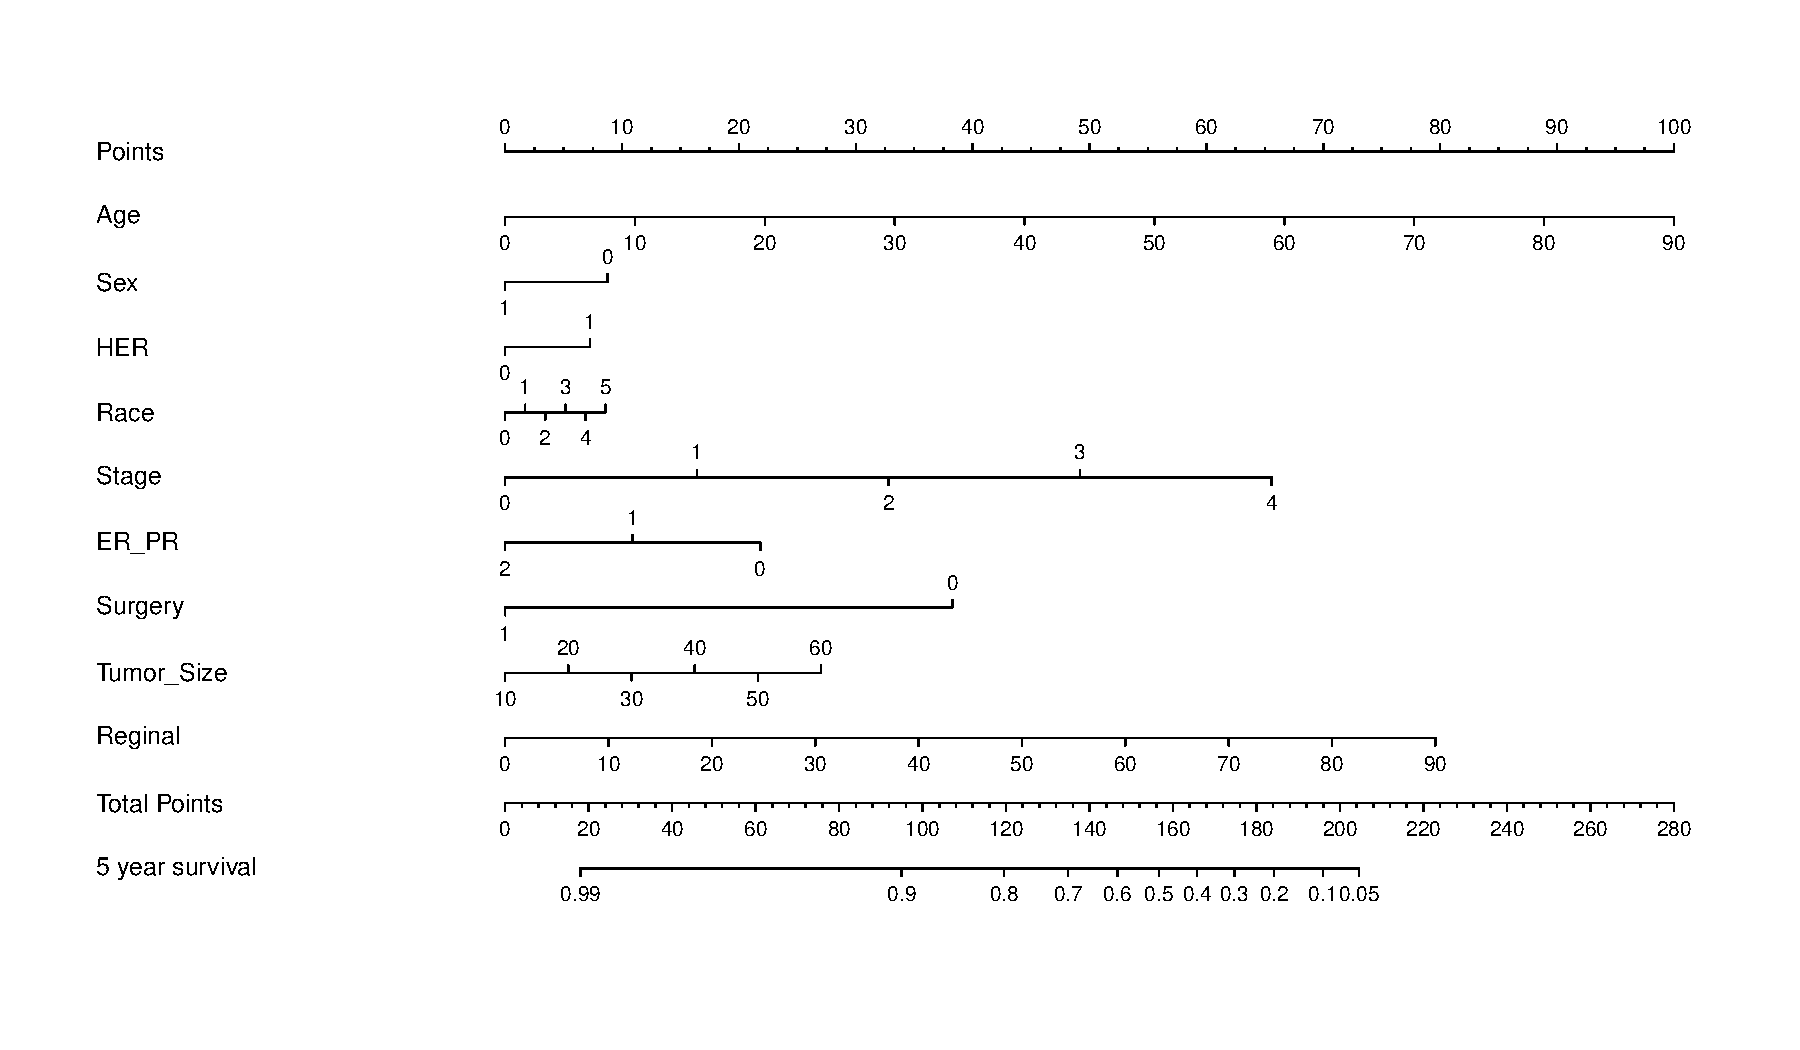
\includegraphics{report_files/figure-latex/unnamed-chunk-3-1.pdf}

The significance of variables is determined by the effect estimates and
is influenced by co-variables. In this figure, age contributes the most
to the outcome thus it is assigned 100 points. In proportion to the most
effective variable, the rest are assigned a point according to their
effect size. Relative importance could be understood by comparing the
most significant variable (Age) to the least significant variable (HER).

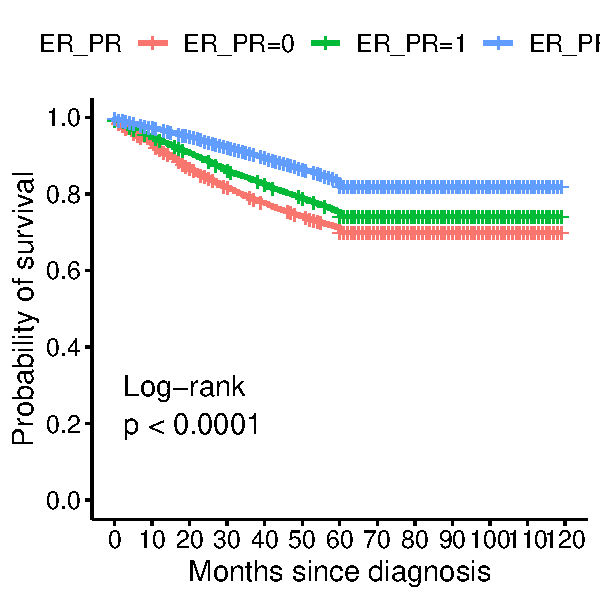
\includegraphics{report_files/figure-latex/unnamed-chunk-4-1.pdf}
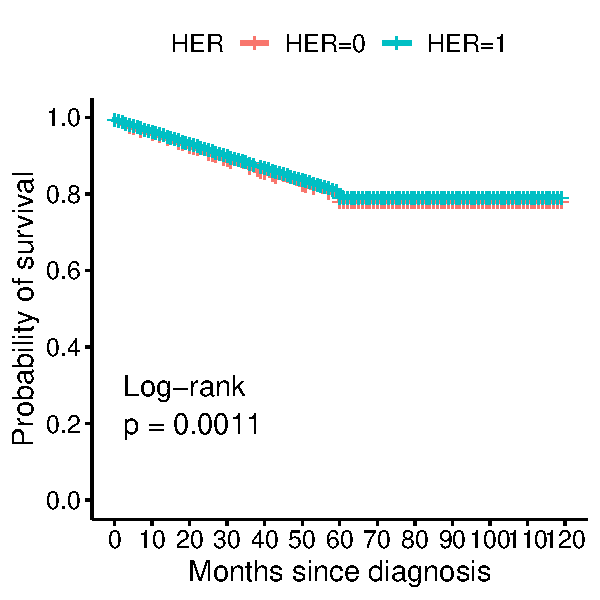
\includegraphics{report_files/figure-latex/unnamed-chunk-4-2.pdf}

Kaplan-Meier plots showed the survival curves using the log-rank test
for the comparison of HER and ER\_PR variables correspondingly. The
p-value in each graph indicates a significant difference in survival
curves among groups. For the ER\_PR variable, three survival curves have
clear separation without intersection. For the HER variable, a
separation is not clear enough, we can still make the inference that a
positive HER indicates a smaller risk of death.

\hypertarget{model-result}{%
\subsubsection{Model Result}\label{model-result}}

The OOB(Out-of-bag) scores for the Cox proportional hazard model and
random forest model are 0.256 and 0.255, which indicates that they
predicted the OOB samples with 74.4\% accuracy and 74.5\% accuracy,
respectively. The C-index calculated from the Cox proportional hazard
model is 0.745 in training data and 0.539 in test data. The C-index
calculated from the random forest model is 0.801 in training data and
0.671 in test data.

\hypertarget{conclusion}{%
\section{Conclusion}\label{conclusion}}

The C-index in both Cox proportional hazard model and the random forest
model is bigger than 0.5, which reflects that they are prediction models
with good fits. And the C-index score of the random survival forest is
higher than the score of the Cox proportional hazard model, which also
indicates that the random survival forest has a higher model fit and
prediction accuracy. Machine learning methods have higher accuracy,
fewer required assumptions, and a higher capacity to deal with big data.
And that's why it was applied in this study. On the other hand, compared
to train data, the C-index in test data is lower. With the development
of treatment, early detection of breast cancer and improved diagnosis
accuracy, there might be bias by using train data from 2004 to 2014 to
predict test data from 2005.

Here are the limitations of the study. The tumor size was observed to be
insignificant, which is inconsistent with previous studies. The effect
of tumor size on survival prediction is associated with the number of
positive lymph nodes(LNs). It has been indicated that small tumors with
more than four positive LNs might be more aggressive diseases compared
to bigger tumors{[}2{]}. In addition, stage I showed an insignificant
result. In previous studies, stage 0 and stage I were combined together
and treated as one reference group because both survival rate is almost
100\%{[}4{]}. That might explain why it's insignificant in this study.

\hypertarget{reference}{%
\section{Reference}\label{reference}}

{[}1{]}Breast cancer statistics: How common is breast cancer? American
Cancer Society. (n.d.). Retrieved December 17, 2022, from
\url{https://www.cancer.org/cancer/breast-cancer/about/how-common-is-breast-cancer.html}

{[}2{]}Liu Y, He M, Zuo WJ, Hao S, Wang ZH, Shao ZM. Tumor Size Still
Impacts Prognosis in Breast Cancer With Extensive Nodal Involvement.
Front Oncol. 2021 Apr 9;11:585613. doi: 10.3389/fonc.2021.585613. PMID:
33898305; PMCID: PMC8064390.

{[}3{]}Balabram D, Turra CM, Gobbi H. Survival of patients with operable
breast cancer (Stages I-III) at a Brazilian public hospital--a closer
look into cause-specific mortality. BMC Cancer. 2013 Sep 24;13:434. doi:
10.1186/1471-2407-13-434. PMID: 24063763; PMCID: PMC3849091.

{[}4{]}Elobaid, Y., Aamir, M., Grivna, M., Suliman, A., Attoub, S.,
Mousa, H., Ahmed, L. A., \& Oulhaj, A. (n.d.). Breast cancer survival
and its prognostic factors in the United Arab Emirates: A retrospective
study. PLOS ONE. Retrieved December 17, 2022, from
\url{https://journals.plos.org/plosone/article?id=10.1371\%2Fjournal.pone.0251118}

{[}5{]}Understanding breast cancer survival rates. Susan G. Komen®.
(2022, July 20). Retrieved December 17, 2022, from
\url{https://www.komen.org/breast-cancer/facts-statistics/breast-cancer-statistics/survival-rates/}

\end{document}
